%
% File acl2012.tex
%
% Contact: Maggie Li (cswjli@comp.polyu.edu.hk), Michael White (mwhite@ling.osu.edu)
%%
%% Based on the style files for ACL2008 by Joakim Nivre and Noah Smith
%% and that of ACL2010 by Jing-Shin Chang and Philipp Koehn


\documentclass[11pt]{article}
\usepackage{acl2012}
\usepackage{times}
\usepackage{latexsym}
\usepackage{amsmath}
\usepackage{multirow}
\usepackage{url}
\DeclareMathOperator*{\argmax}{arg\,max}
\setlength\titlebox{6.5cm}    % Expanding the titlebox

\title{Detecting English Writing Styles For Non Native Speakers}

\author{Rami Al-Rfou', Yanging Chen, Yejin Choi \\
  Department of Computer Science \\
  Stony Brook University \\
  NY 11794, USA \\
  {\tt \{ralrfou, cyanqing, ychoi\}@cs.stonybrook.edu}}

\date{12/15/2011}

\usepackage{graphicx}
\begin{document}
\maketitle
\begin{abstract}
%Rami's Part
%Explain what is our target of whole project.
\end{abstract}


\section{Introduction}
%Rami's Part

\section{Related Work}
%Chen's part
%Mentions what people did, and how our work is different and original.

The first work related with native language identification is that of \newcite {Koppel:2005}, in which they tried profiling anonymous authors with their native languages. Totally five different groups of English authors (whose native languages are Russian, Bulgarian, French, and Spanish) were picked from the first version of {\em International Corpus of Learner English} (ICLE) in their experiments. By applying a combined feature sets, including function words, character n-grams, part-of-speech bi-grams and spelling mistakes, they gained an accuracy of 65\% if considered style features only. These results suggested that syntactic features are valuable when trying to categorize authors by their native languages.  

Similar work was done by \newcite {Tsur:2007}. They focused on the relationships between choice of words in second language writing and the frequency of native language syllables, also known as the phonology of native languages. And \newcite {Estival:2007}. studied a wide range of lexical and document structure features in their native laguages classification task. But either of these two measured the usefulness of syntacitc features for the task of native language detection.

\newcite {Wong:2009} replicated the work of \newcite {Koppel:2005} and digged more in the field of syntactic stuctures. They experimented on three selected syntactic errors, which are commonly observed in non-native English Users, including subject-verb disagreement, mismatch of noun-number pairs and wrong usage of determiners and the best overall accuracy was 73.71\% on the second version of ICLE across seven languages. What's more, \newcite {Wong:2011} continued their works in native language detection and focused more on the influence of syntactic structures, specifically parsing trees. They tried to exploiting the parsing structures by applying Standford parsers and C\&J parsers with different parameters to certain corpus, and capture the number of usages of some distinguishable rules. Their results and observations suggested that the syntactic structures would be supportive in detecting native languages and improving the performance of existing classifiers.

Different from previous works mentioned above, our task runs on a totally different platform--wikipedia. Our goal is to find out the influence of one's native languages on the style of his/her writings under the circumstance of talking and discussion. With the help of huge amount of available data, we can try exploring the statistics features of a certain languages using similar features in \newcite {Koppel:2005} and \newcite {Wong:2011}, as well as the distribution of part-of-speech n-grams and word n-grams.      

\section{Wikipedia}
%Explain why wikipedia is an awesome source
%Explain wikipedia structure
%Explain how there are two different ways to get users contributions
%Explain the comments extraction algorithm
%Rami's Part

Wikipedia is the de facto source of knowledge for internet users. Wikipedia is the 5\textsuperscript{th} most popular website according to Google ranking. For researchers Wikipedia is a giant linguistic and social jar of experiments. The richness of the website content that is written by users from different backgrounds represents a robust sample of the current languages usage by native and non native speakers.

With more than 90 thousand active users and 4.4 million article the content of Wikipedia spans large number of topics. The diversity of the authors of those articles beside the records of the revisions that are stored in a database of revisions that the website offer for free presents a realistic source of text. Such resource presents a higher quality of data that is not achievable by the other commonly used sources of text as news and scientific papers.

Such successful website has a complex database structure to serve its users. Therefore, extracting data could be a complex process. Our goal is to identify the languages skills of the users and collect their contributions. To achieve the first task Wikipedia has a an information box called \emph{Babel} that users can add voluntarily to their profile pages to state their skills in different languages. Figure \ref{babel} shows a user who identified his native language and her skills in 3 other non native languages in a scale for 1-5. This info box will be indexed in the database as categories.


\begin{figure}[htp]
\centering
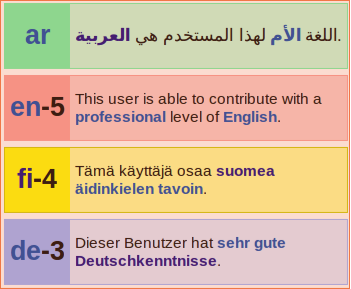
\includegraphics[scale=0.60]{babel}
\caption{Wikipedia languages skills info box (Babel)}
\label{babel}
\end{figure}

To collect the contributions of a specific user the task is more complex procedure. The diffs between Wikipedia pages revisions has to be generated and linked back to the user table. However, the resources we have to process such huge amount of data did not allow us to do that\footnote{Recent efforts were made to generate the diffs \url{http://dumps.wikimedia.org/other/diffdb/}}. Instead we noticed that Wikipedia pages have accompanying discussion pages where users discuss different aspects of the articles. In those pages the tradition is to sign the user comments with a signature that link back to the user. Figure \ref{obama} shows the style of the writing of those talk pages are less formal and technical than the main pages of Wikipedia and has more conversational stylistic features.

\begin{figure*}[Htp]
\centering
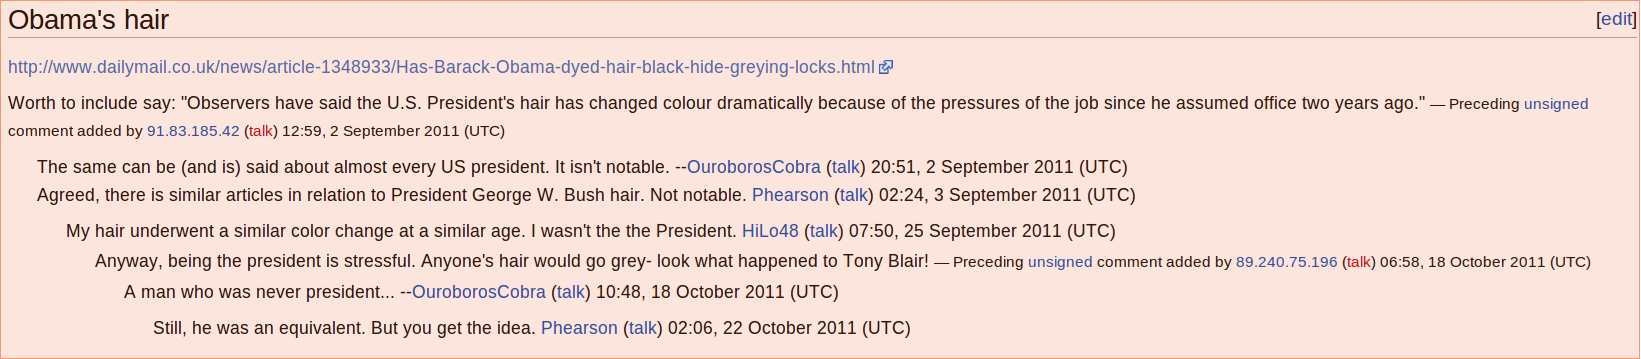
\includegraphics[scale=0.285]{obama.png}
\caption{Example of a conversation in the discussion pages}
\label{obama}
\end{figure*}

The patterns of the recommended signatures styles are limited in number, however, in practice the users use various patterns that makes the detection rules ambiguous. The detection algorithm implemented relies on complex regular expressions and applies best effort strategy.



\section{Experiments}
%Rami's part
We found that around 60 thousands users specified their language skills. Figure \ref{native_dist} shows that the percentage of users who claimed that their one of their native languages is English is around 47\% of English wikipedia users base. 
\begin{figure}[htp]
\centering
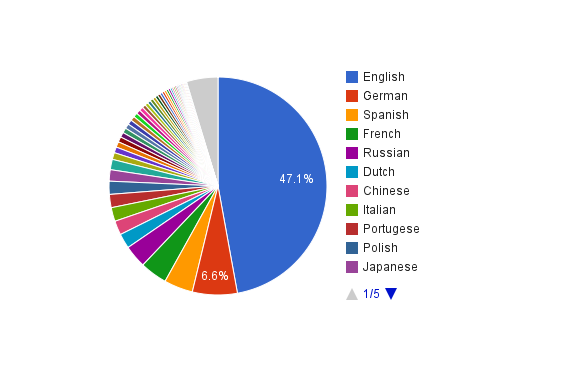
\includegraphics[scale=0.5]{chart_4.png}
\caption{Users distribution over native languages in English Wikipedia}
\label{native_dist}
\end{figure}

We parsed the talk pages with the \verb+namespace=1+, they represents x\% of the talk pages, which produced around 12 million comments. Only 2.4 million comment we could identify to users with known language skills. Moreover, not all the users made comments in the talk pages we parsed, therefore, The number of the users who made at least one contribution in the extracted contributions is around 30 thousand user.

As we have large number of comments and users and as we believe the data we have is still noisy. We applied the following filtering mechanisms:
\begin{itemize}
\item We picked the users of the most popular 20 native languages.
\item We picked out of the English native speakers the users who specified the EN-US as their native language only to avoid users who are so skilled in English but are not living in English speaking countries.
\item We excluded the users who specified more than one native language out of the picked native languages to avoid unrealistic scenarios where users claim to be native in more than two languages.
\end{itemize}

The new data set after the filtering is consistent of 9857 user and 589228 comments.

\subsection{Setup}
%Explain the pruning and the filtering that was done to the data.
The following experiments are conducted under the following conditions:
\begin{itemize}
\item The accepted comments has to have at least 20 tokens to avoid short and non meaningful comments.
\item Proper nouns are replaced by their tags to avoid bias toward topics.
\item Non ascii characters are replaced by a special character to avoid bias foreign languages usage in the comments.
\item The classifier has balanced number of samples for each its classes.
\item Logistic Regression algorithm is used to for the classification task.
\item The data set is split to 70\% training set, 10\% development set and 20\% testing set.
\end{itemize}

\subsection{Features}
The comments of training set is grouped by class and the following language models are calculated for each class:
\begin{itemize}
\item
\end{itemize}

We calculated the 1-4 grams over the words


\subsection{Popular Languages Experiment}
%Explain the experiment and the results

\begin{figure}[htp]
\centering
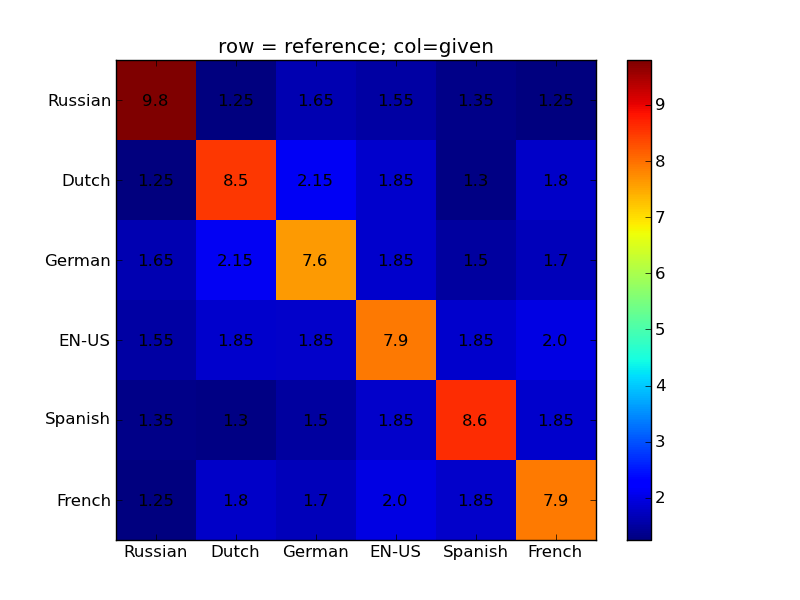
\includegraphics[scale=0.45]{popular_cfm.png}
\caption{Popular Languages experiment confusion matrix}
\label{pop_cfm}
\end{figure}

\begin{figure}[htp]
\centering
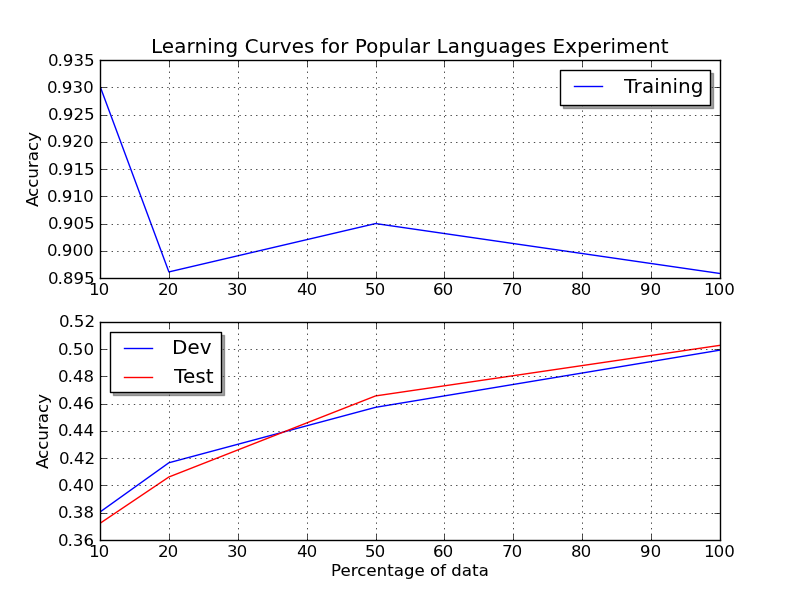
\includegraphics[scale=0.45]{popular_lc.png}
\caption{Popular languages experiment learning curves}
\label{pop_lc}
\end{figure}
		
\subsection{Languages Families Experiment}
%Explain the experiment and the results
\begin{figure}[htp]
\centering
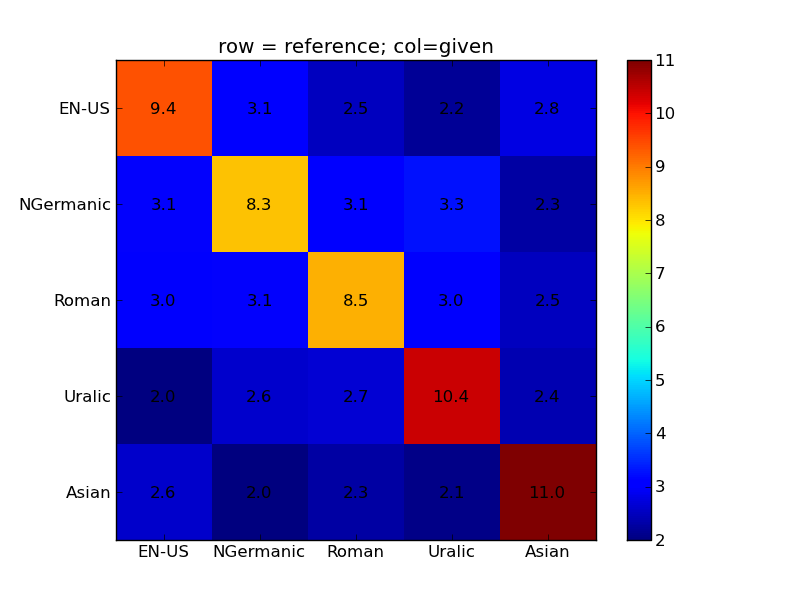
\includegraphics[scale=0.45]{family_cfm.png}
\caption{Languages families experiment confusion matrix}
\label{fam_cfm}
\end{figure}

\begin{figure}[htp]
\centering
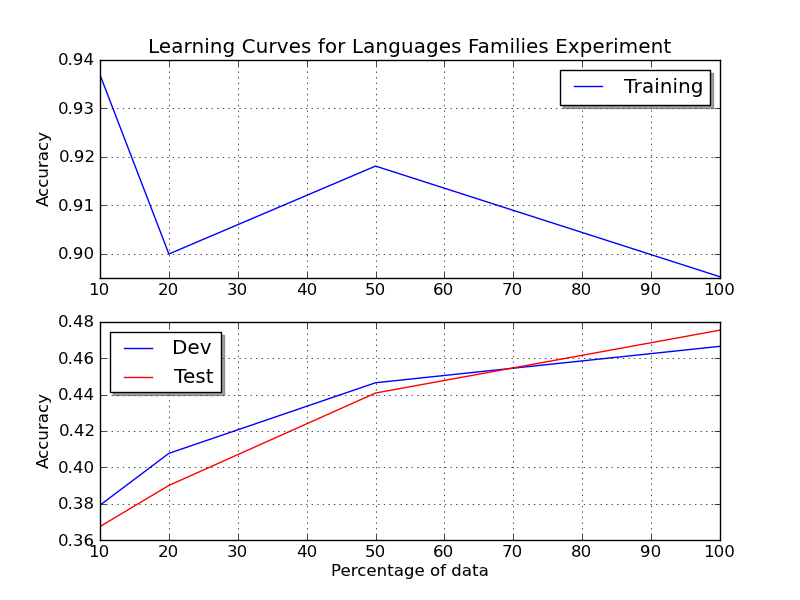
\includegraphics[scale=0.45]{family_lc.png}
\caption{Languages families experiment learning curves}
\label{fam_lc}
\end{figure}

\subsection{Native vs Non Native Experiment}
%Explain the experiment and the results
\begin{figure}[htp]
\centering
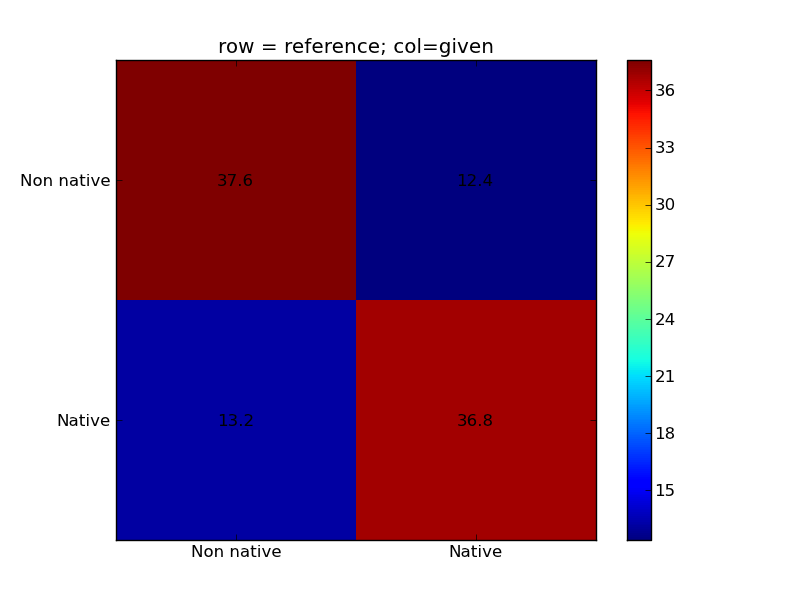
\includegraphics[scale=0.45]{native_cfm.png}
\caption{Native vs Non Native speakers experiment confusion matrix}
\label{non_cfm}
\end{figure}

\begin{figure}[htp]
\centering
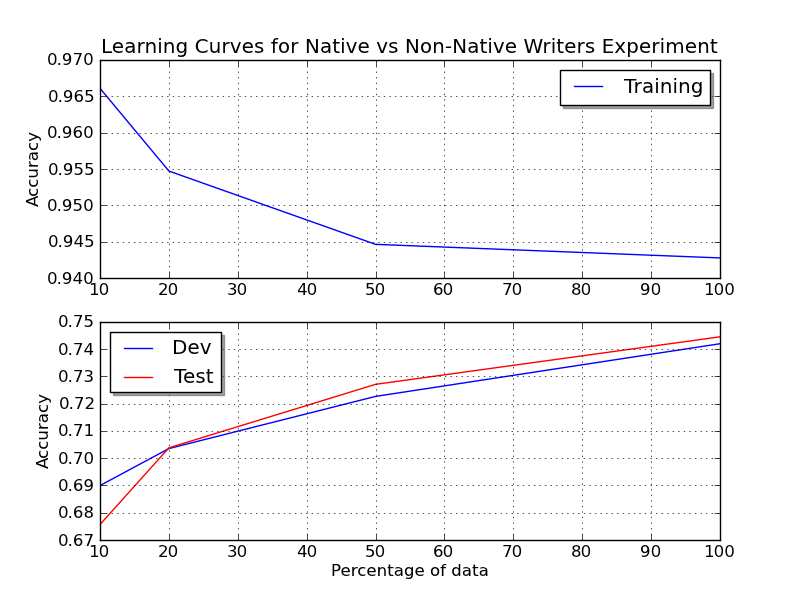
\includegraphics[scale=0.45]{native_lc.png}
\caption{Non native vs native experiment learning curves}
\label{non_lc}
\end{figure}

\section{Writing Styles}
%Chen's part


\section{Conclusions}
%Chen's Part

\section*{Acknowledgments}
%Chen's Part
%We should thank Prof. Skiena for the resources he gave us.

\begin{thebibliography}{}

\bibitem[\protect\citename{Estival \bgroup et al.\egroup}2007]{Estival:2007}
Dominique Estival, Tanja Gaustad, Son-Bao Pham, Will Radford, and Ben Hutchinson.
\newblock 2007.
\newblock Author profiling for English emails. In {\em Proceedings of the 10th Conference of the Pacific Association for Computational Linguistics (PACLING)}, pages 263-272.

\bibitem[\protect\citename{Koppel \bgroup et al.\egroup}2005]{Koppel:2005}
Moshe Koppel, Jonathan Schler, and Kfir Zigdon.
\newblock 2005.
\newblock Automatically determining an anonymous author’s native language. In {\em Intelligence and Security Informatics}, volume 3495 of {\em Lecture Notes in Computer Science}, pages 209-217.
\newblock Springer-Verlag.

\bibitem[\protect\citename{Tsur and Rappoport}2007]{Tsur:2007}
Oren Tsur and Ari Rappoport.
\newblock 2007.
\newblock Using classifier features for studying the effect of native language on the choice of written second language words. In {\em Proceedings of the Workshop on Cognitive Aspects of Computational Language Acquisition}, pages 9-16.

\bibitem[\protect\citename{{Wong and Dras}}2009]{Wong:2009}
Sze-Meng Jojo Wong and Mark Dras.
\newblock 2009.
\newblock Contrastive analysis and native language identification. In {\em Proceedings of the Australasian Language Technology As sociation Workshop 2009}, pages 53-61.
\newblock Sydney, Australia, December.

\bibitem[\protect\citename{Wong and Dras}2011]{Wong:2011}
Sze-Meng Jojo Wong and Mark Dras.
\newblock 2011.
\newblock Exploiting Parse Structures for Native Language Identification. In {\em Proceedings of the 2011 Conference on Empirical Methods in Natural Language Processing}, pages 1600–1610.
\newblock Edinburgh, Scotland, UK.

\end{thebibliography}

\end{document}
